% ============================================
% 附录
% ============================================
\section{附录 A：核心数据模型定义}

\subsection{用户认证模型}

\begin{minted}[linenos]{typescript}
model User {
  id            String    @id @default(cuid())
  name          String?
  email         String    @unique
  emailVerified DateTime?
  image         String?
  password      String?
  createdAt     DateTime  @default(now())
  updatedAt     DateTime  @updatedAt

  accounts       Account[]
  sessions       Session[]
  authenticators Authenticator[]
  surveys        Survey[]
  collaborations SurveyCollaborator[]
  surveyLogs     SurveyLog[]
}

model Account {
  id                String  @id @default(cuid())
  userId            String
  type              String
  provider          String
  providerAccountId String
  refresh_token     String? @db.Text
  access_token      String? @db.Text
  expires_at        Int?
  token_type        String?
  scope             String?
  id_token          String? @db.Text
  session_state     String?

  user User @relation(fields: [userId], references: [id], onDelete: Cascade)
  @@unique([provider, providerAccountId])
}
\end{minted}
\captionof{listing}{User 与 Account 模型}

\begin{minted}[linenos]{typescript}
model Session {
  id           String   @id @default(cuid())
  sessionToken String   @unique
  userId       String
  expires      DateTime
  user User @relation(fields: [userId], references: [id], onDelete: Cascade)
}

model Authenticator {
  credentialID         String  @unique
  userId               String
  providerAccountId    String
  credentialPublicKey  String
  counter              Int
  credentialDeviceType String
  credentialBackedUp   Boolean
  transports           String?
  user User @relation(fields: [userId], references: [id], onDelete: Cascade)
  @@unique([userId, credentialID])
}
\end{minted}
\captionof{listing}{Session 与 Authenticator 模型}

\subsection{问卷核心模型}

\begin{minted}[linenos]{typescript}
model Survey {
  id               String   @id @default(cuid())
  title            String
  description      String?
  published        Boolean  @default(false)
  shareToken       String   @unique @default(cuid())
  settings         Json?
  userId           String
  maxCollaborators Int      @default(10)
  currentVersionId String?
  createdAt        DateTime @default(now())
  updatedAt        DateTime @updatedAt

  user          User                 @relation(fields: [userId], references: [id], onDelete: Cascade)
  questions     Question[]
  responses     Response[]
  views         SurveyView[]
  collaborators SurveyCollaborator[]
  invites       SurveyInvite[]
  logs          SurveyLog[]
  versions      SurveyVersion[]
  @@index([currentVersionId])
}

model Question {
  id          String       @id @default(cuid())
  surveyId    String
  type        QuestionType
  title       String
  description String?
  required    Boolean      @default(false)
  order       Int
  config      Json?
  lockedBy    String?
  lockedAt    DateTime?
  survey  Survey   @relation(fields: [surveyId], references: [id], onDelete: Cascade)
  answers Answer[]
  @@index([lockedBy])
}
\end{minted}
\captionof{listing}{问卷与题目模型}

\begin{minted}[linenos]{typescript}
model SurveyVersion {
  id          String   @id @default(cuid())
  surveyId    String
  version     Int
  title       String
  description String?
  questions   Json
  publishedAt DateTime @default(now())
  createdAt   DateTime @default(now())
  survey    Survey     @relation(fields: [surveyId], references: [id], onDelete: Cascade)
  responses Response[]
  @@unique([surveyId, version])
  @@index([surveyId])
  @@index([publishedAt])
}

model Response {
  id          String   @id @default(cuid())
  surveyId    String
  versionId   String
  respondent  String?
  startedAt   DateTime?
  completedAt DateTime?
  createdAt   DateTime @default(now())
  survey  Survey        @relation(fields: [surveyId], references: [id], onDelete: Cascade)
  version SurveyVersion @relation(fields: [versionId], references: [id], onDelete: Cascade)
  answers Answer[]
  @@index([versionId])
  @@index([createdAt])
}

model Answer {
  id         String @id @default(cuid())
  responseId String
  questionId String
  value      Json
  response Response @relation(fields: [responseId], references: [id], onDelete: Cascade)
  question Question @relation(fields: [questionId], references: [id], onDelete: Cascade)
}
\end{minted}
\captionof{listing}{版本与回答模型}

\clearpage
\subsection{协作与日志模型}

\begin{minted}[linenos]{typescript}
model SurveyCollaborator {
  id             String @id @default(cuid())
  surveyId       String
  userId         String
  canEdit        Boolean @default(false)
  canViewResults Boolean @default(false)
  invitedBy      String
  createdAt      DateTime @default(now())
  survey Survey @relation(fields: [surveyId], references: [id], onDelete: Cascade)
  user   User   @relation(fields: [userId], references: [id], onDelete: Cascade)
  @@unique([surveyId, userId])
  @@index([surveyId])
  @@index([userId])
}

model SurveyInvite {
  id          String    @id @default(cuid())
  surveyId    String
  code        String    @unique
  maxUses     Int?
  usedCount   Int       @default(0)
  expiresAt   DateTime?
  permissions Json?
  createdBy   String
  createdAt   DateTime  @default(now())
  survey Survey @relation(fields: [surveyId], references: [id], onDelete: Cascade)
  @@index([surveyId])
  @@index([code])
}
\end{minted}
\captionof{listing}{协作者与邀请码模型}

\begin{minted}[linenos]{typescript}
model SurveyLog {
  id        String   @id @default(cuid())
  surveyId  String
  userId    String
  action    String
  details   Json?
  createdAt DateTime @default(now())
  survey Survey @relation(fields: [surveyId], references: [id], onDelete: Cascade)
  user   User   @relation(fields: [userId], references: [id], onDelete: Cascade)
  @@index([surveyId])
  @@index([createdAt])
}

model SurveyView {
  id         String   @id @default(cuid())
  surveyId   String
  viewedAt   DateTime @default(now())
  ip         String?
  deviceType String?
  os         String?
  browser    String?
  country    String?
  province   String?
  city       String?
  survey Survey @relation(fields: [surveyId], references: [id], onDelete: Cascade)
  @@index([surveyId])
  @@index([viewedAt])
}
\end{minted}
\captionof{listing}{操作日志与浏览记录模型}

\section{附录 B：系统界面截图}

\begin{figure}[H]
\centering
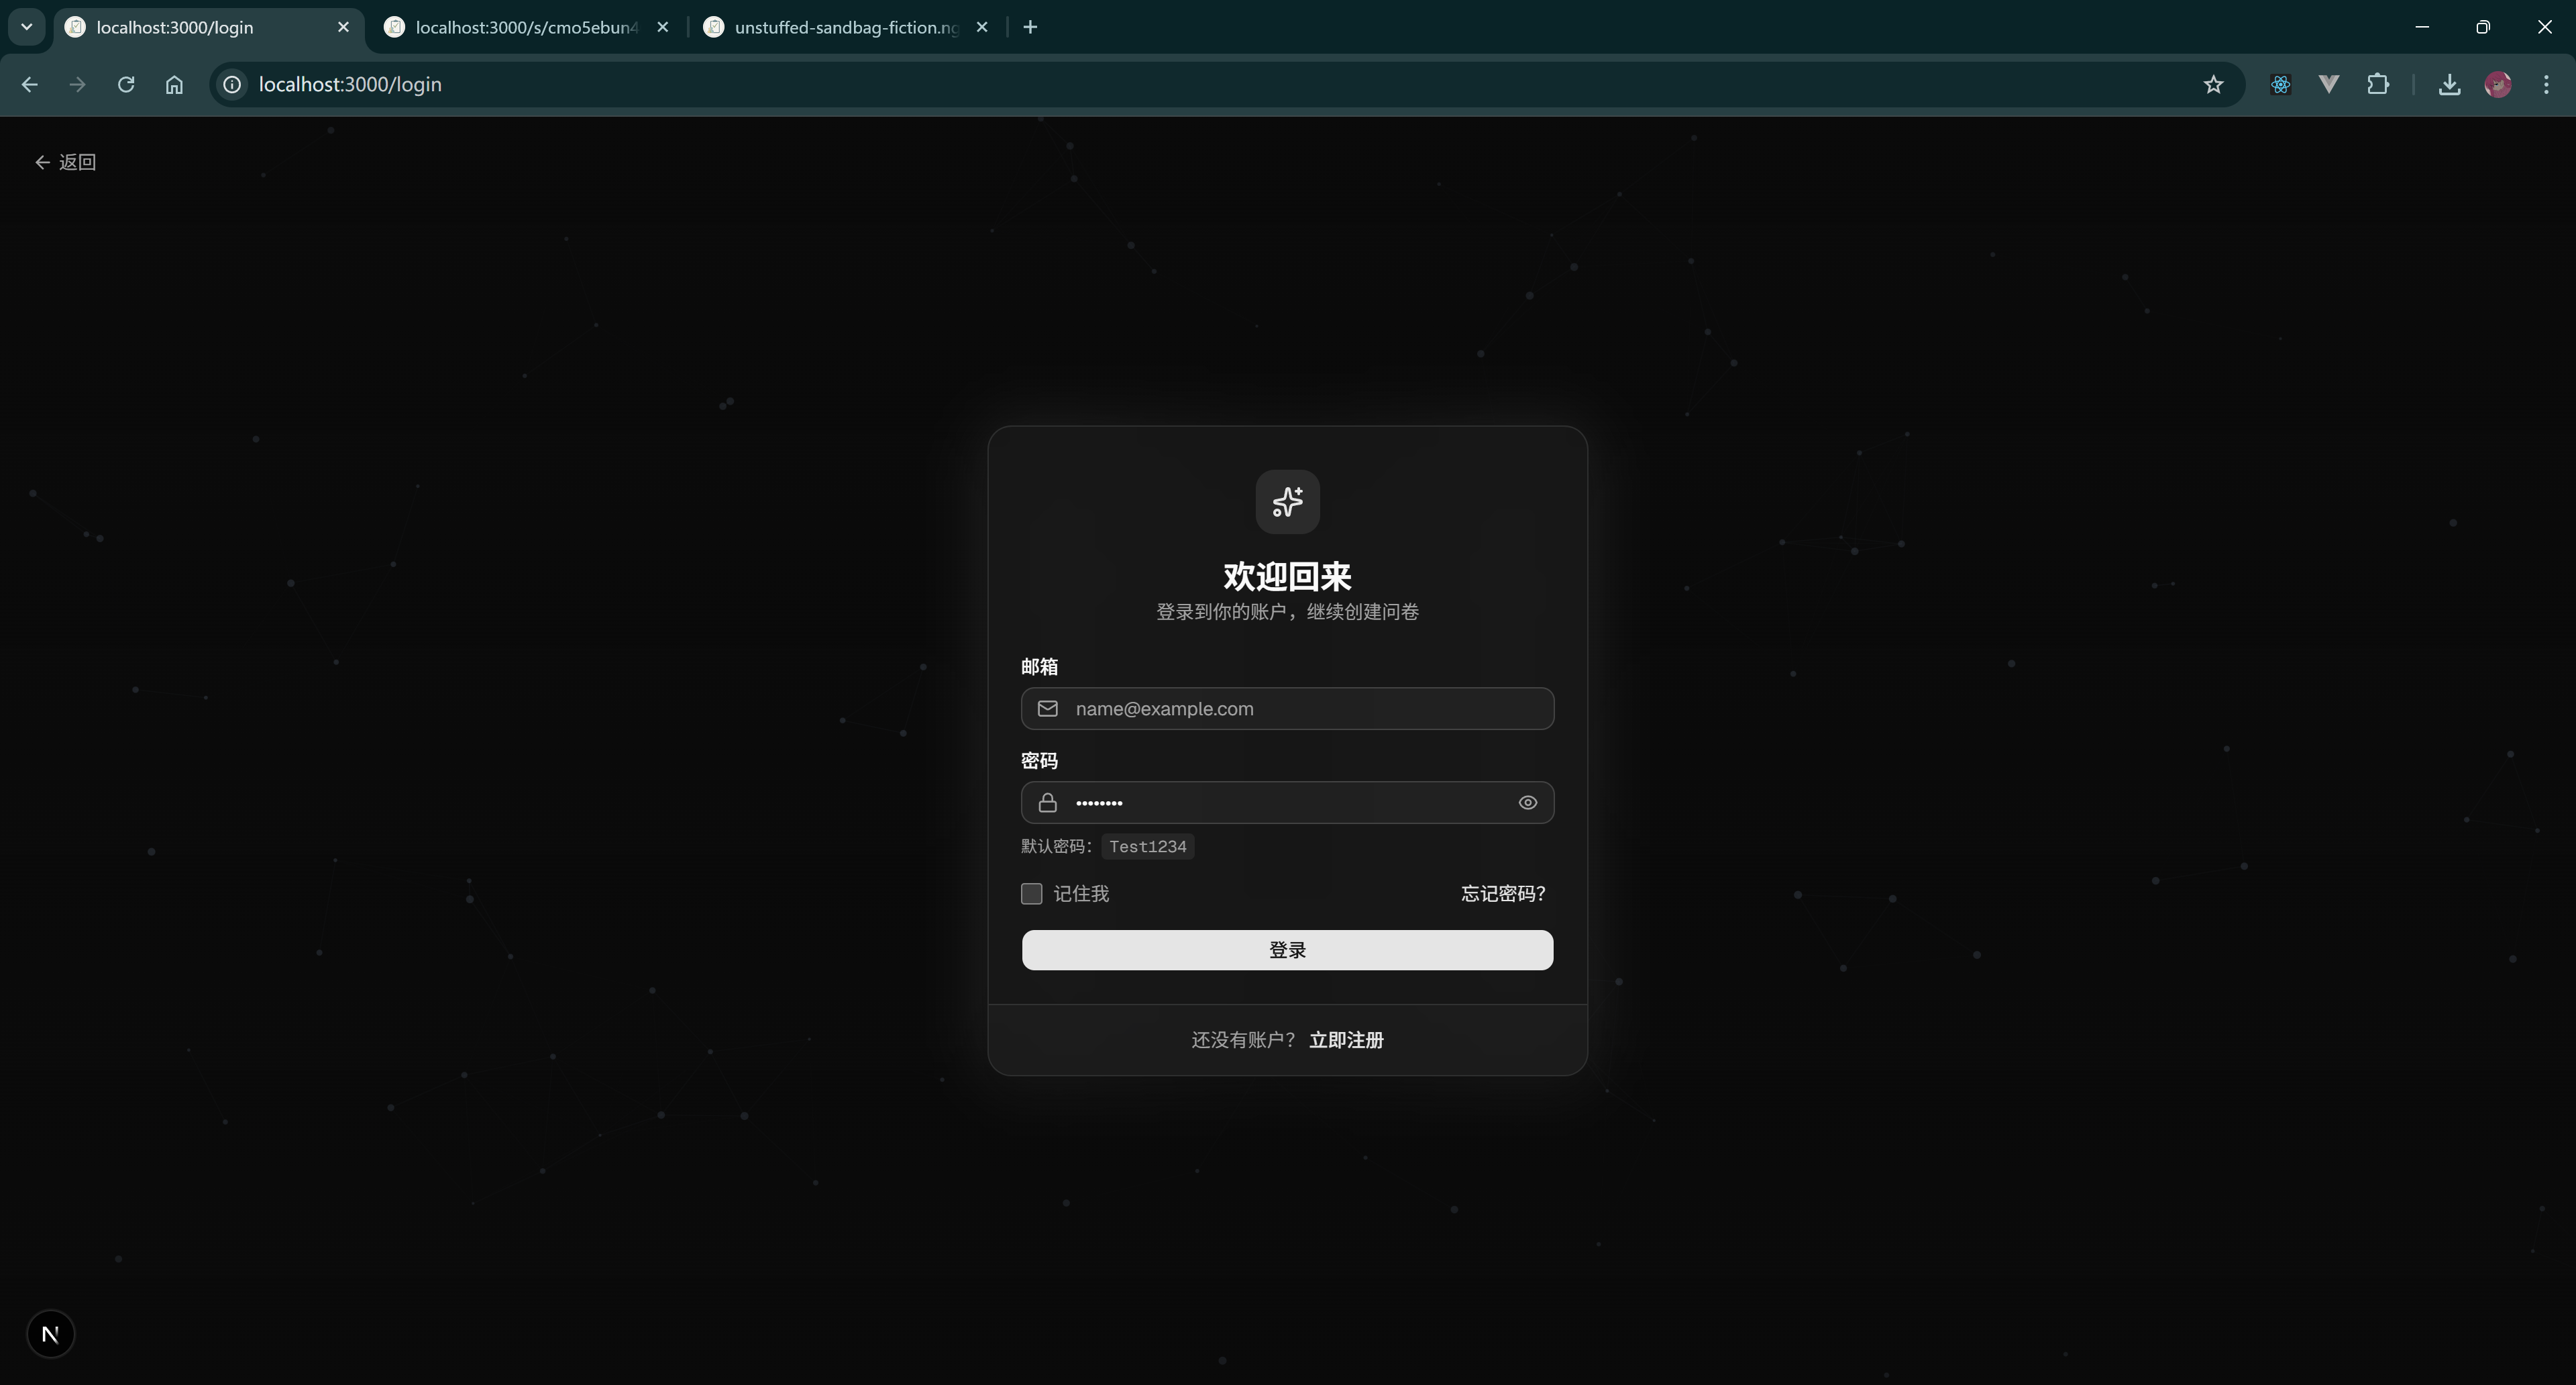
\includegraphics[width=0.95\textwidth]{figures/screenshot-login.png}
\caption{登录页面}
\end{figure}

\begin{figure}[H]
\centering
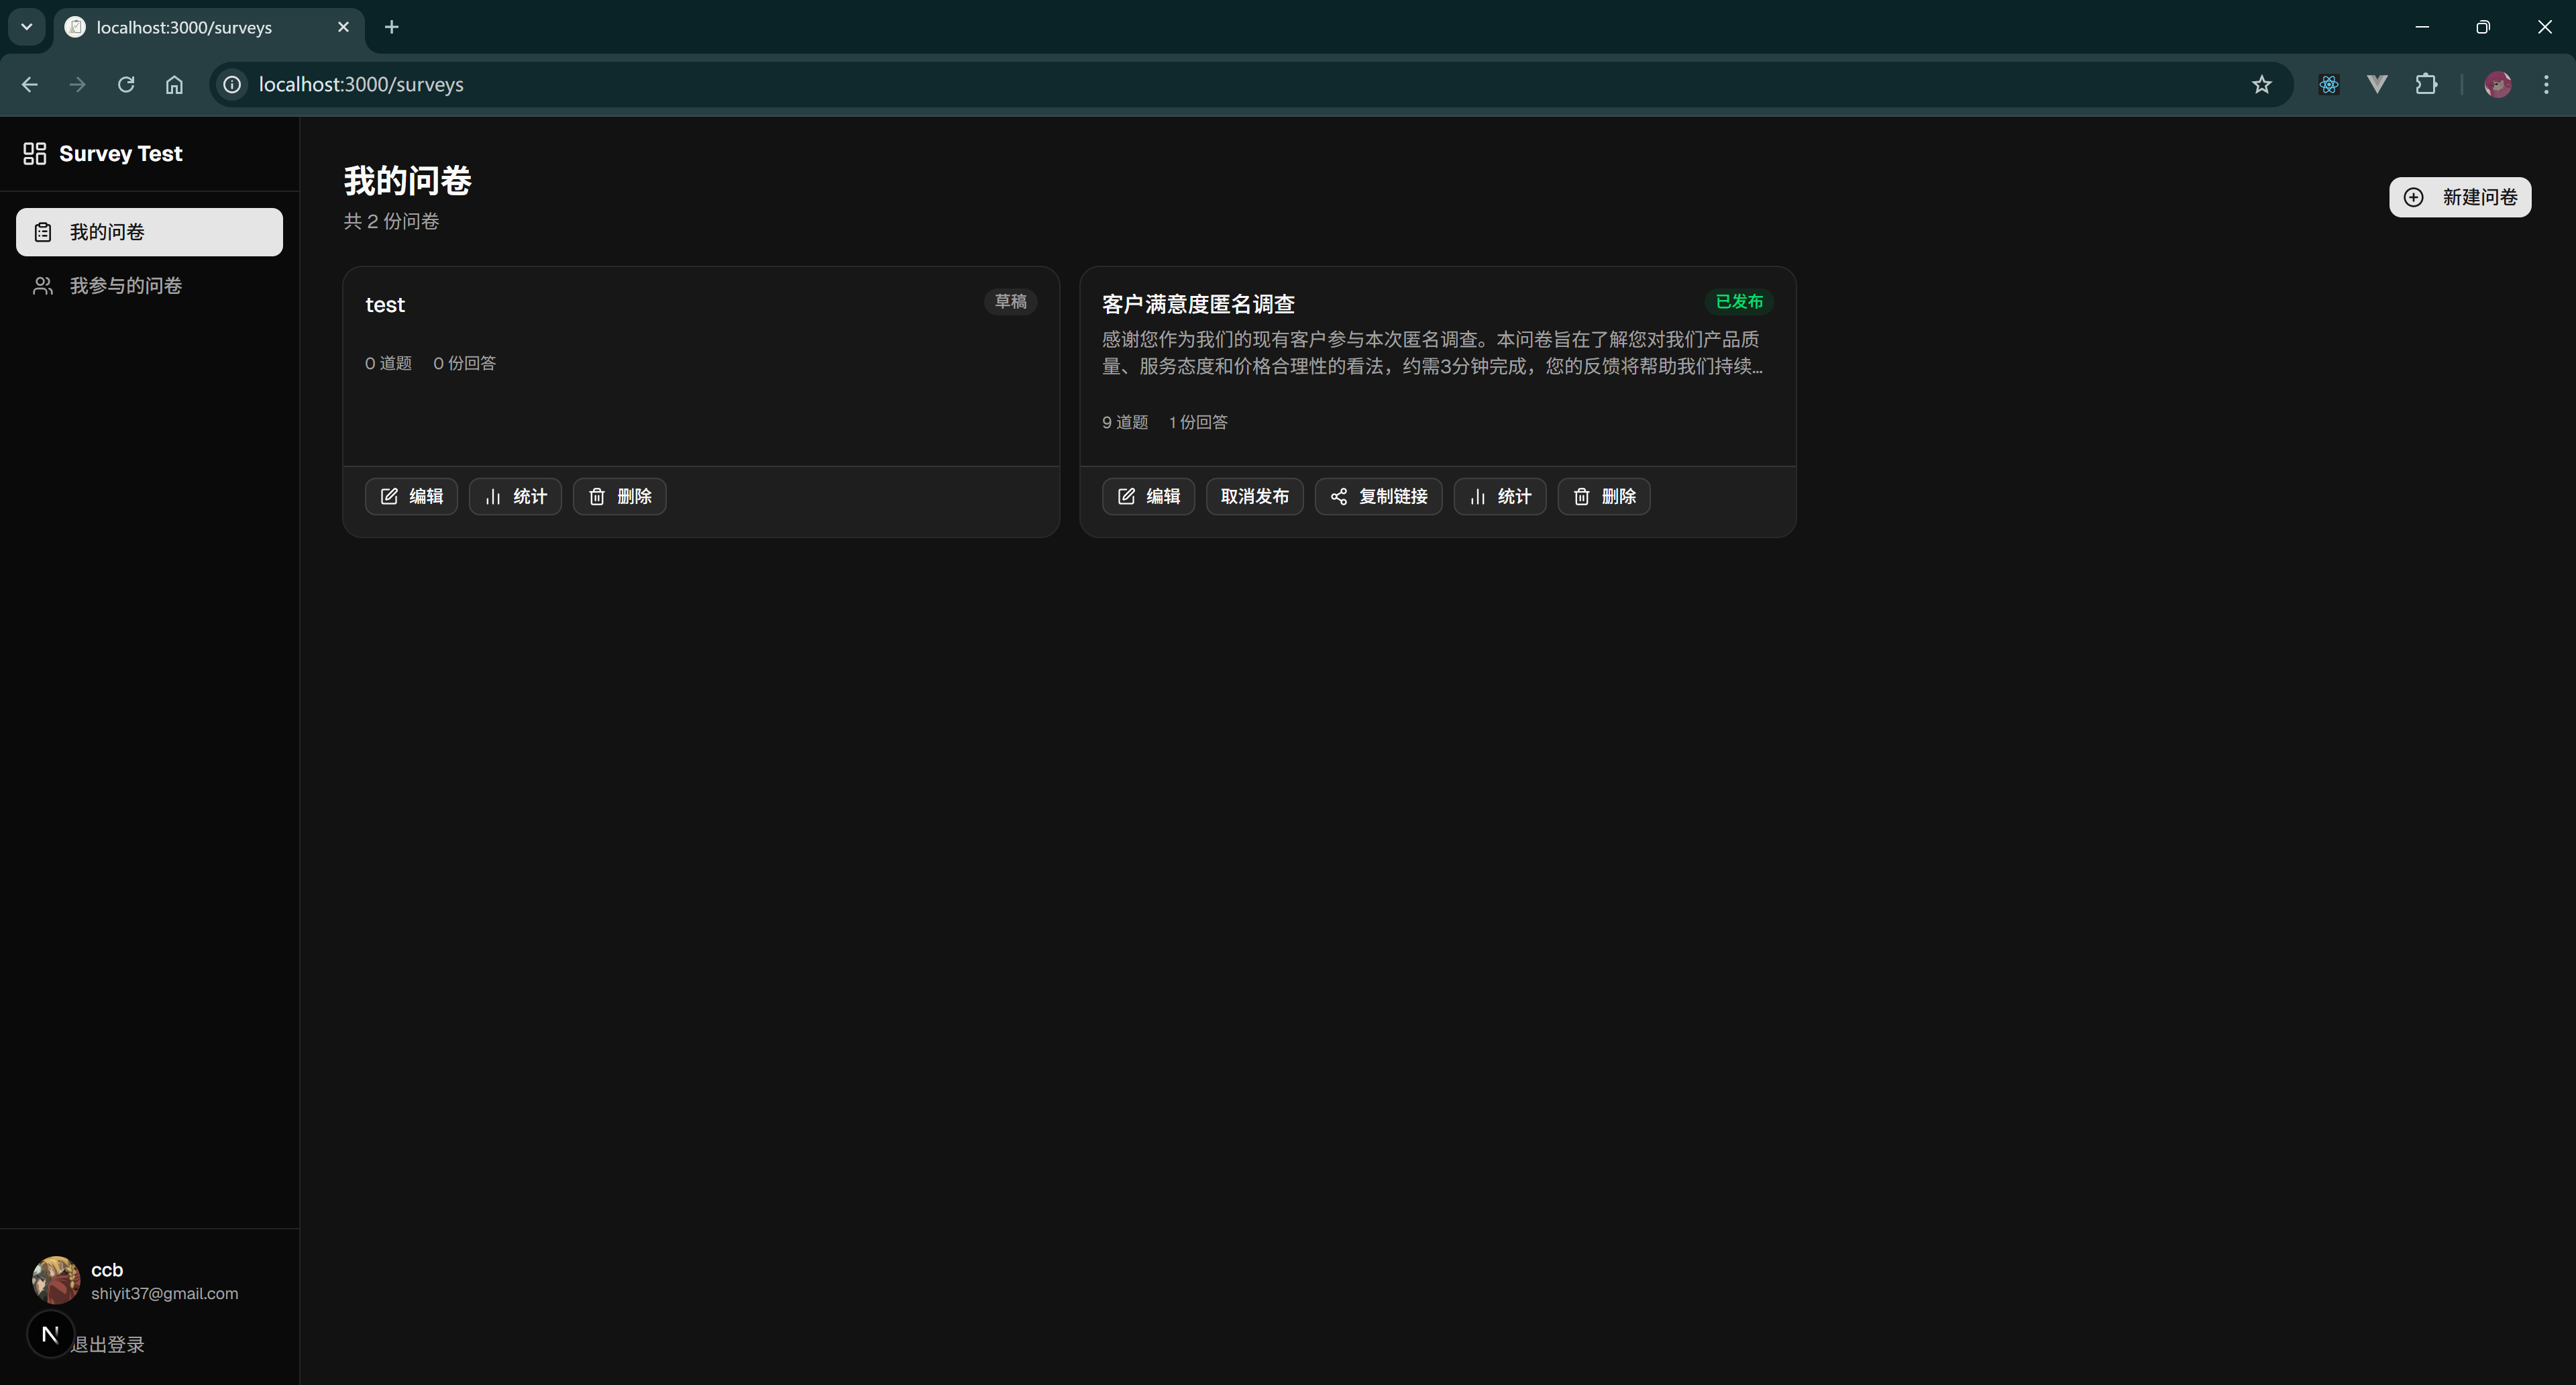
\includegraphics[width=0.95\textwidth]{figures/screenshot-survey-list.png}
\caption{问卷列表页面}
\end{figure}

\begin{figure}[H]
\centering
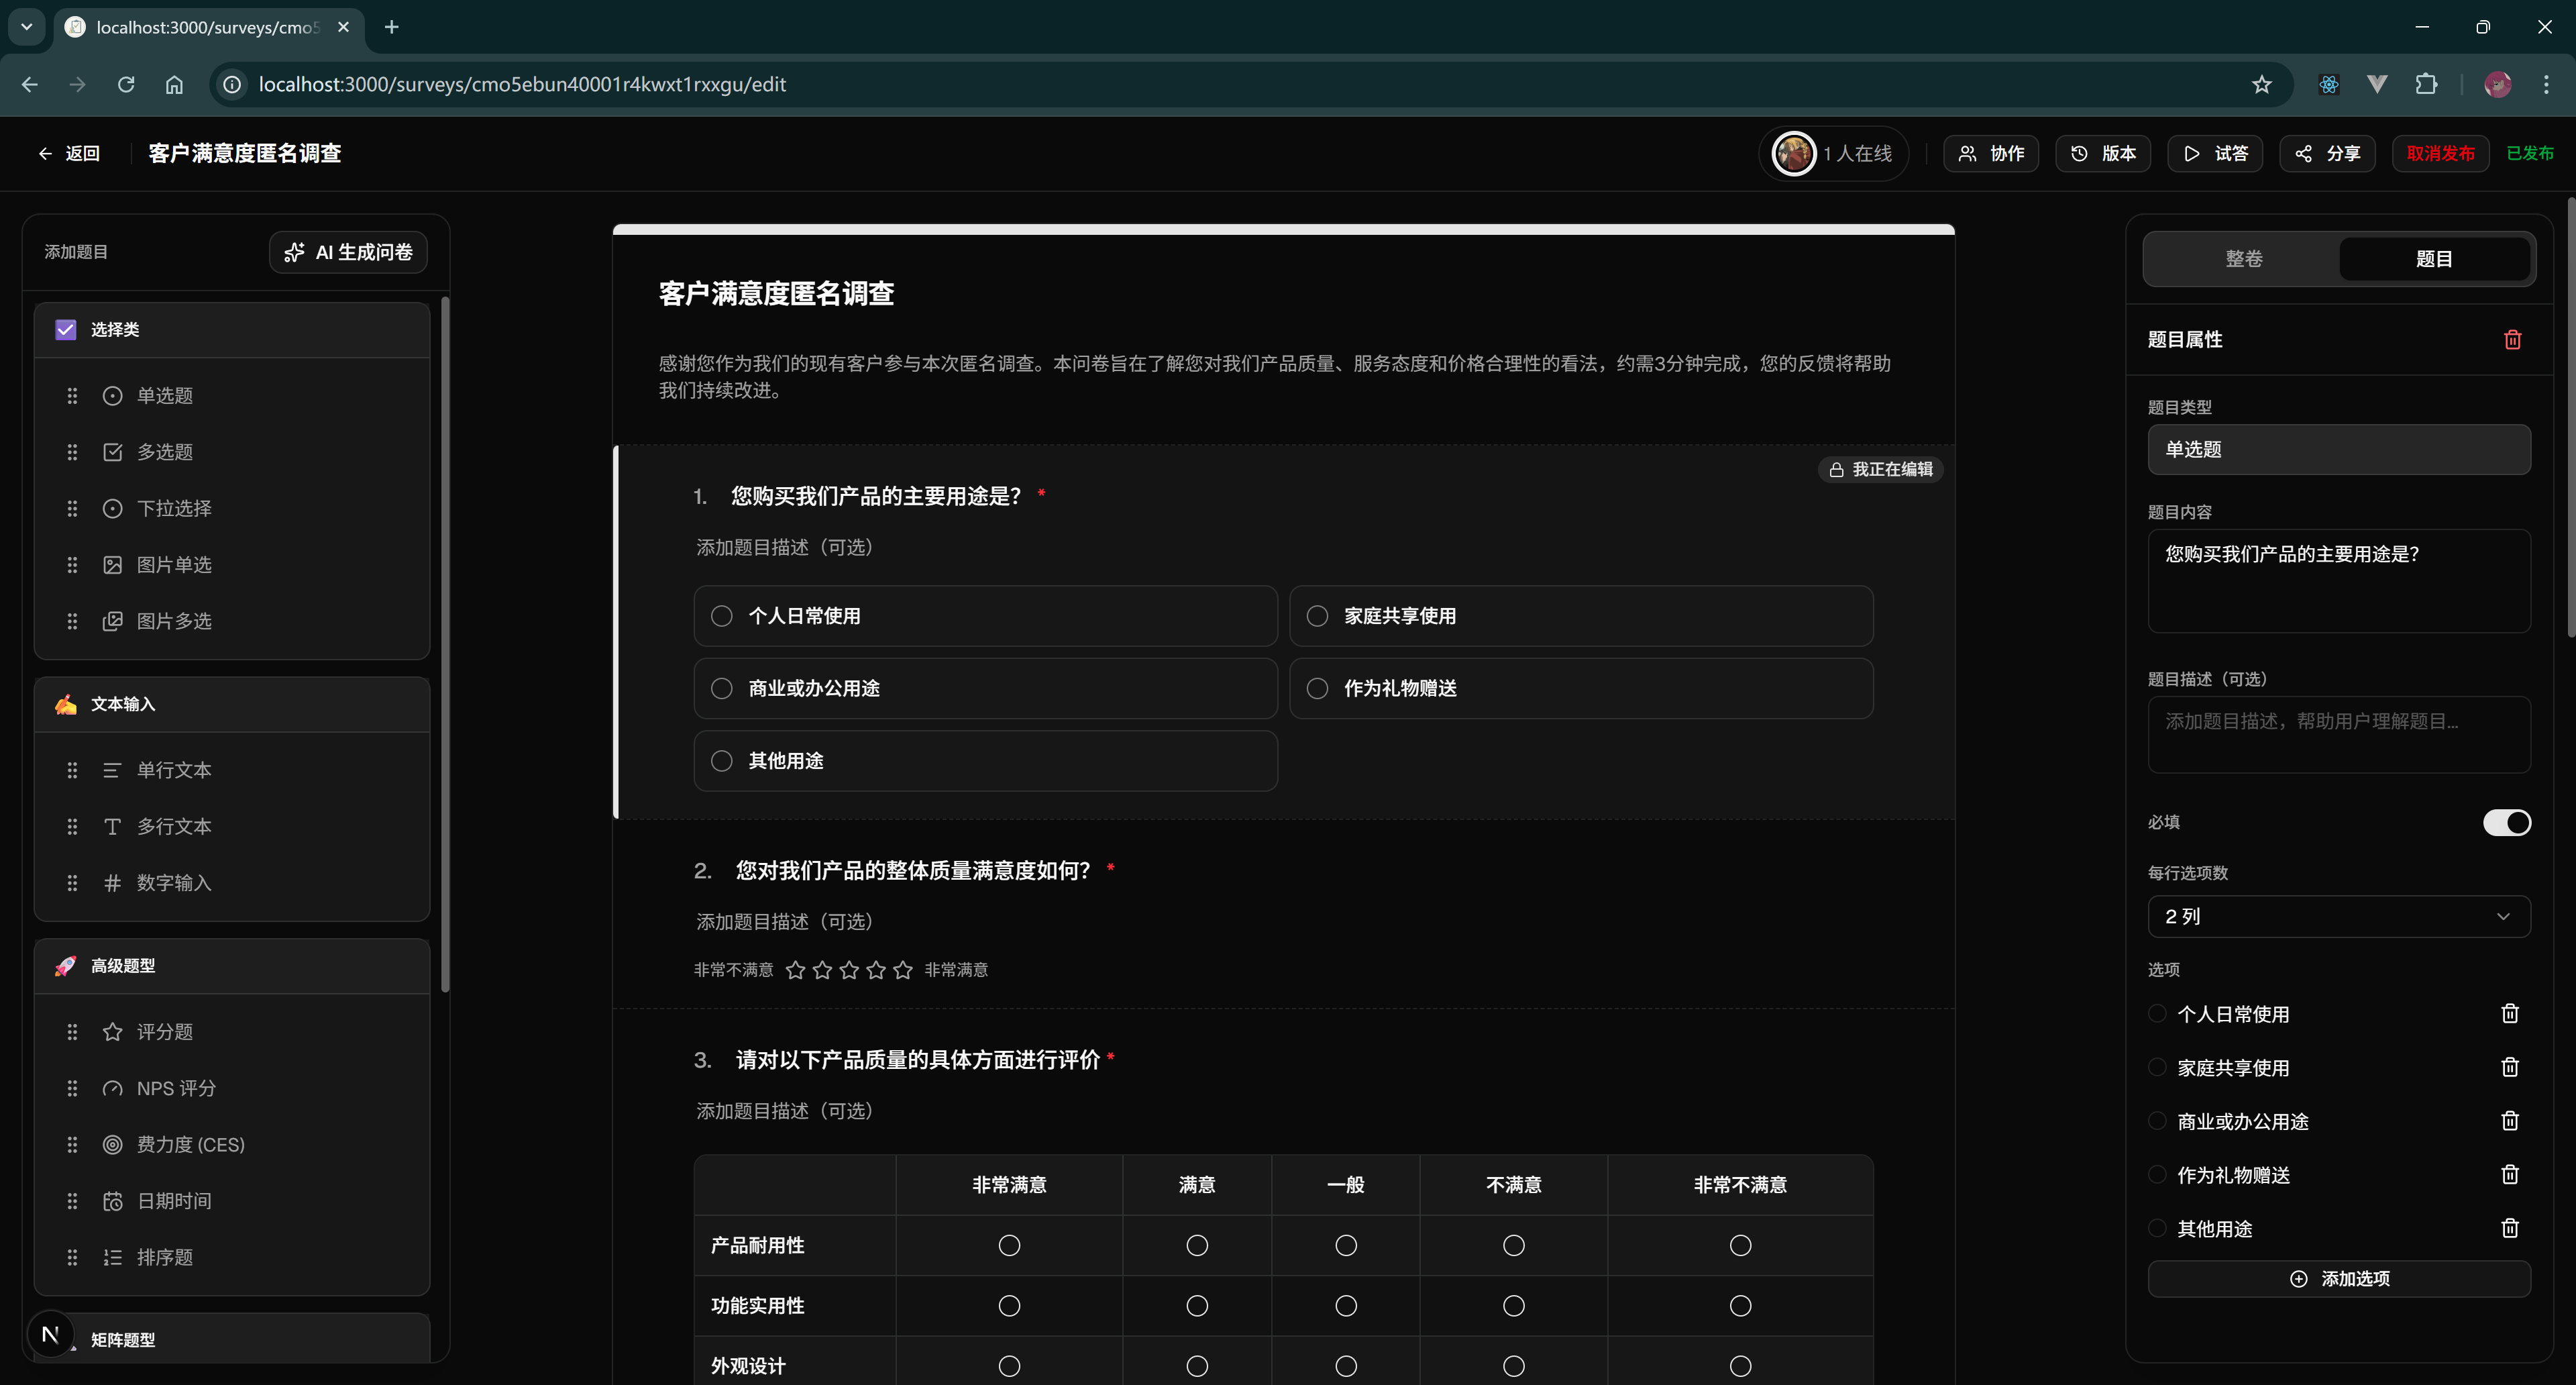
\includegraphics[width=0.95\textwidth]{figures/screenshot-editor.png}
\caption{问卷编辑器}
\end{figure}

\begin{figure}[H]
\centering
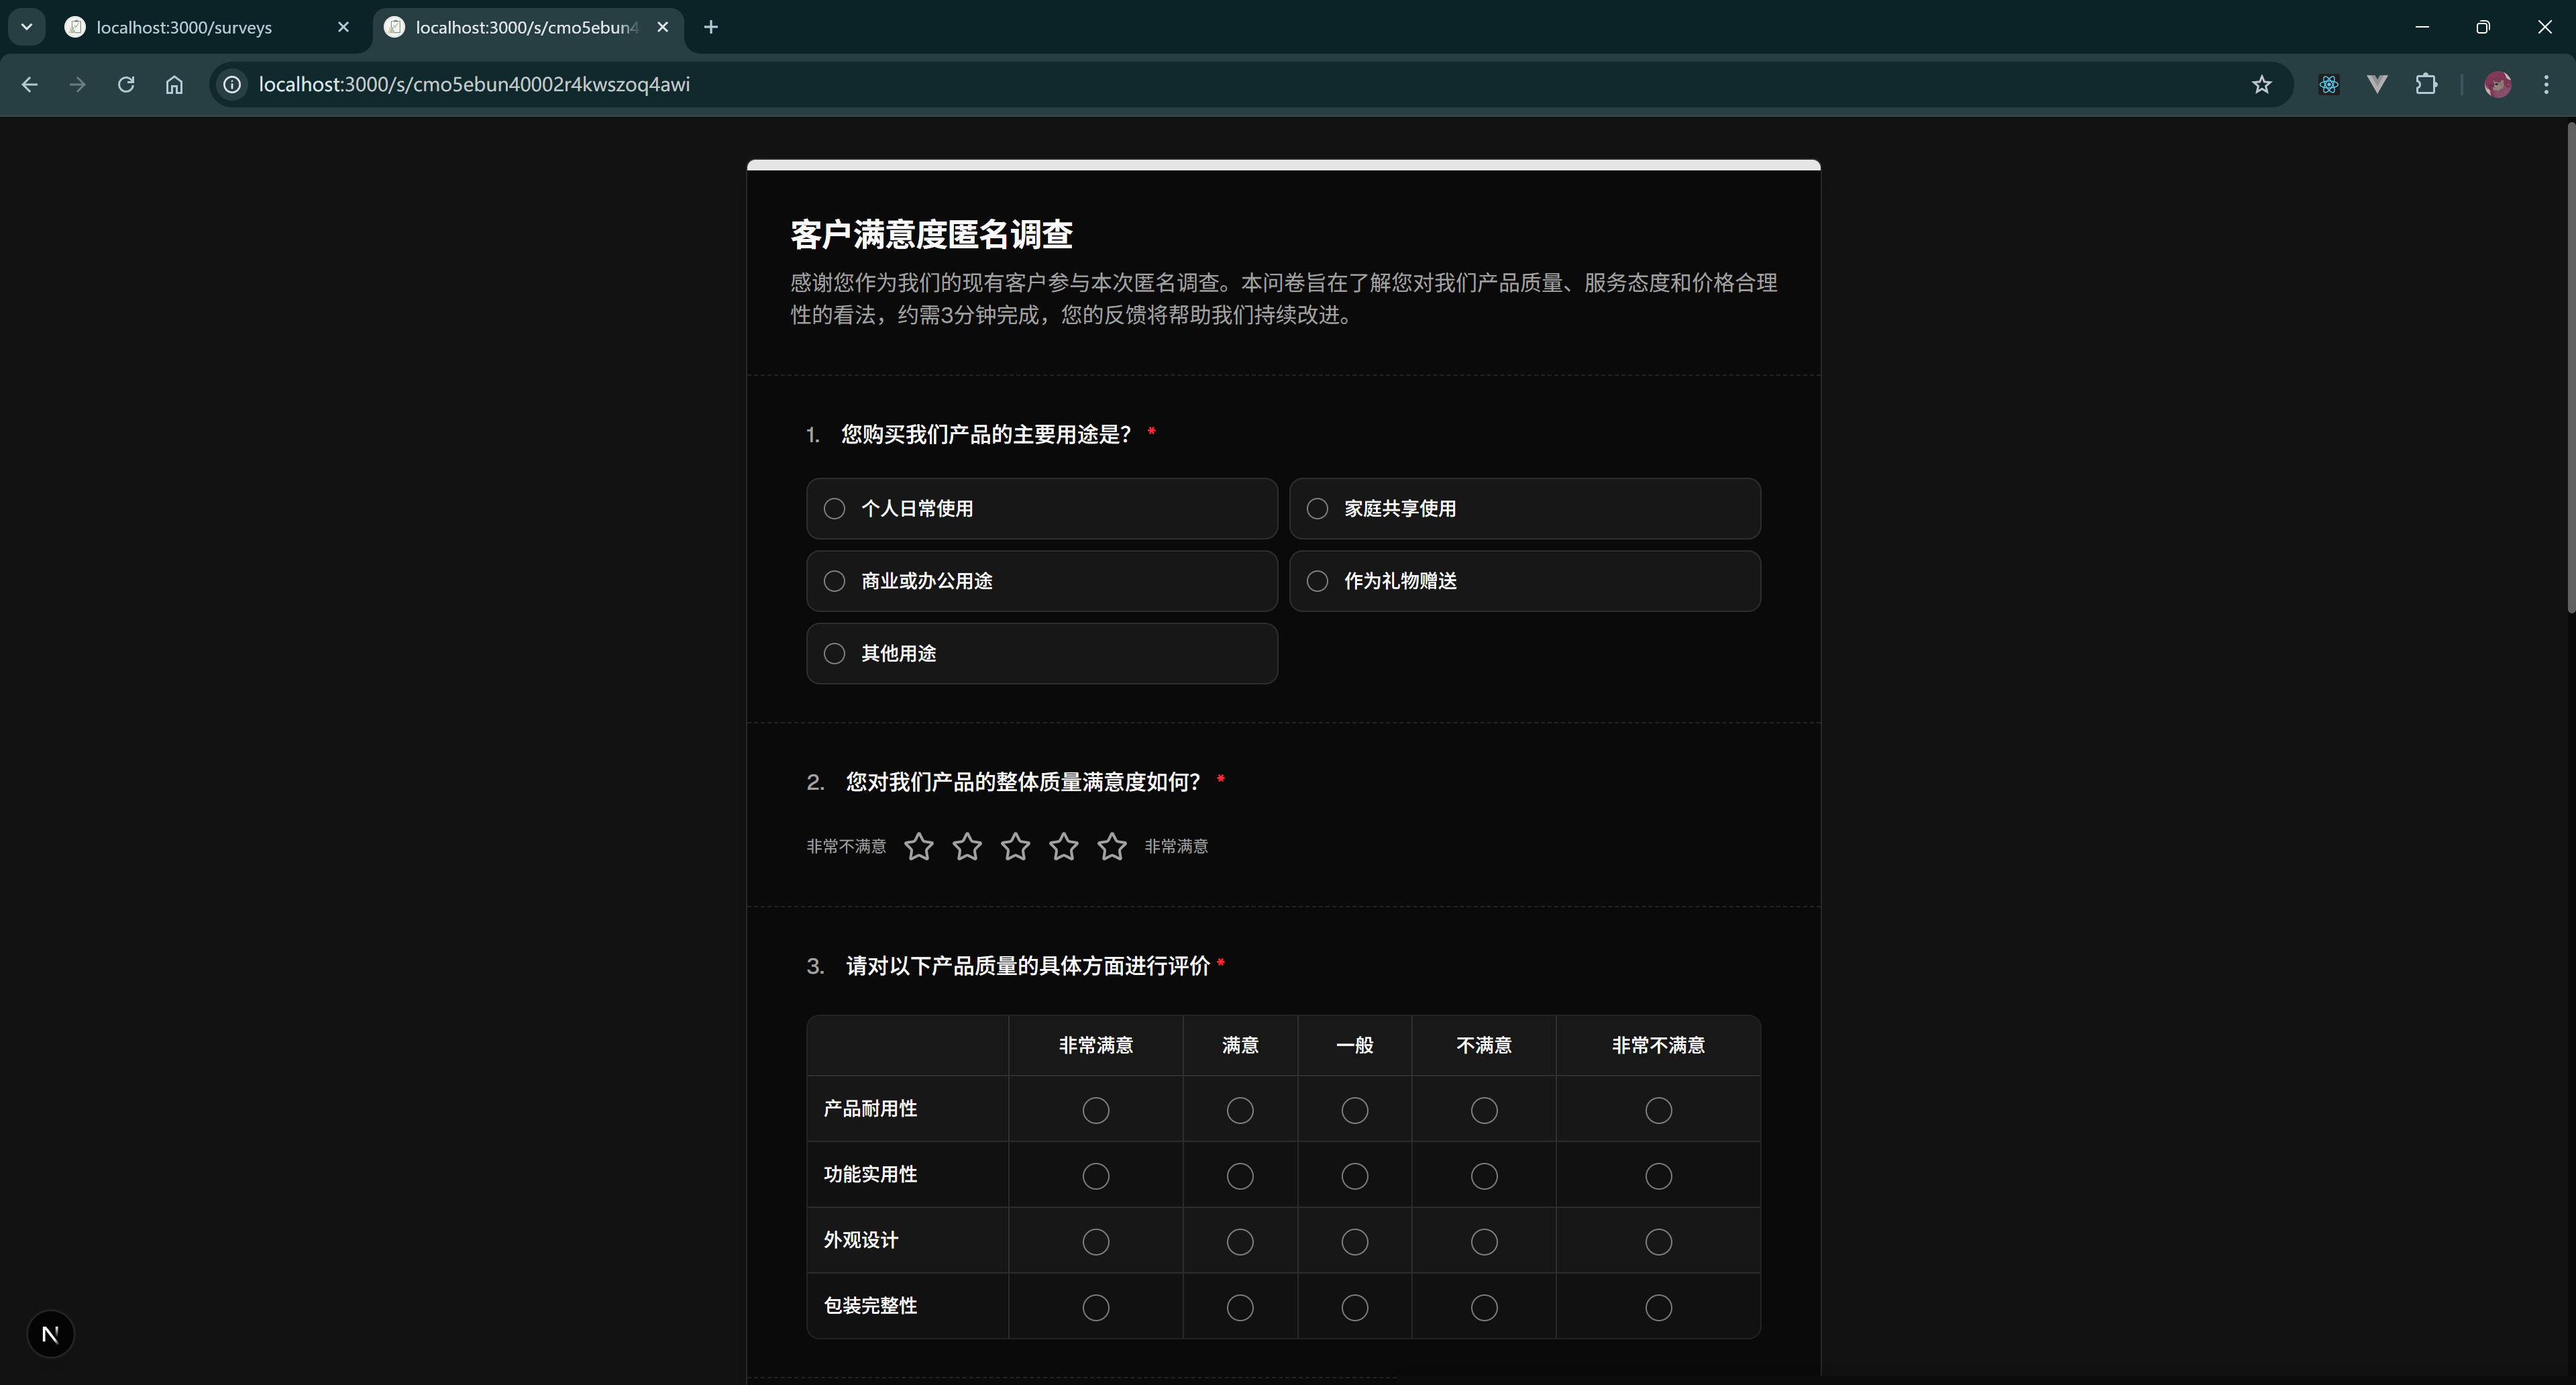
\includegraphics[width=0.95\textwidth]{figures/screenshot-public-form.png}
\caption{公开问卷填写页面}
\end{figure}

\begin{figure}[H]
\centering
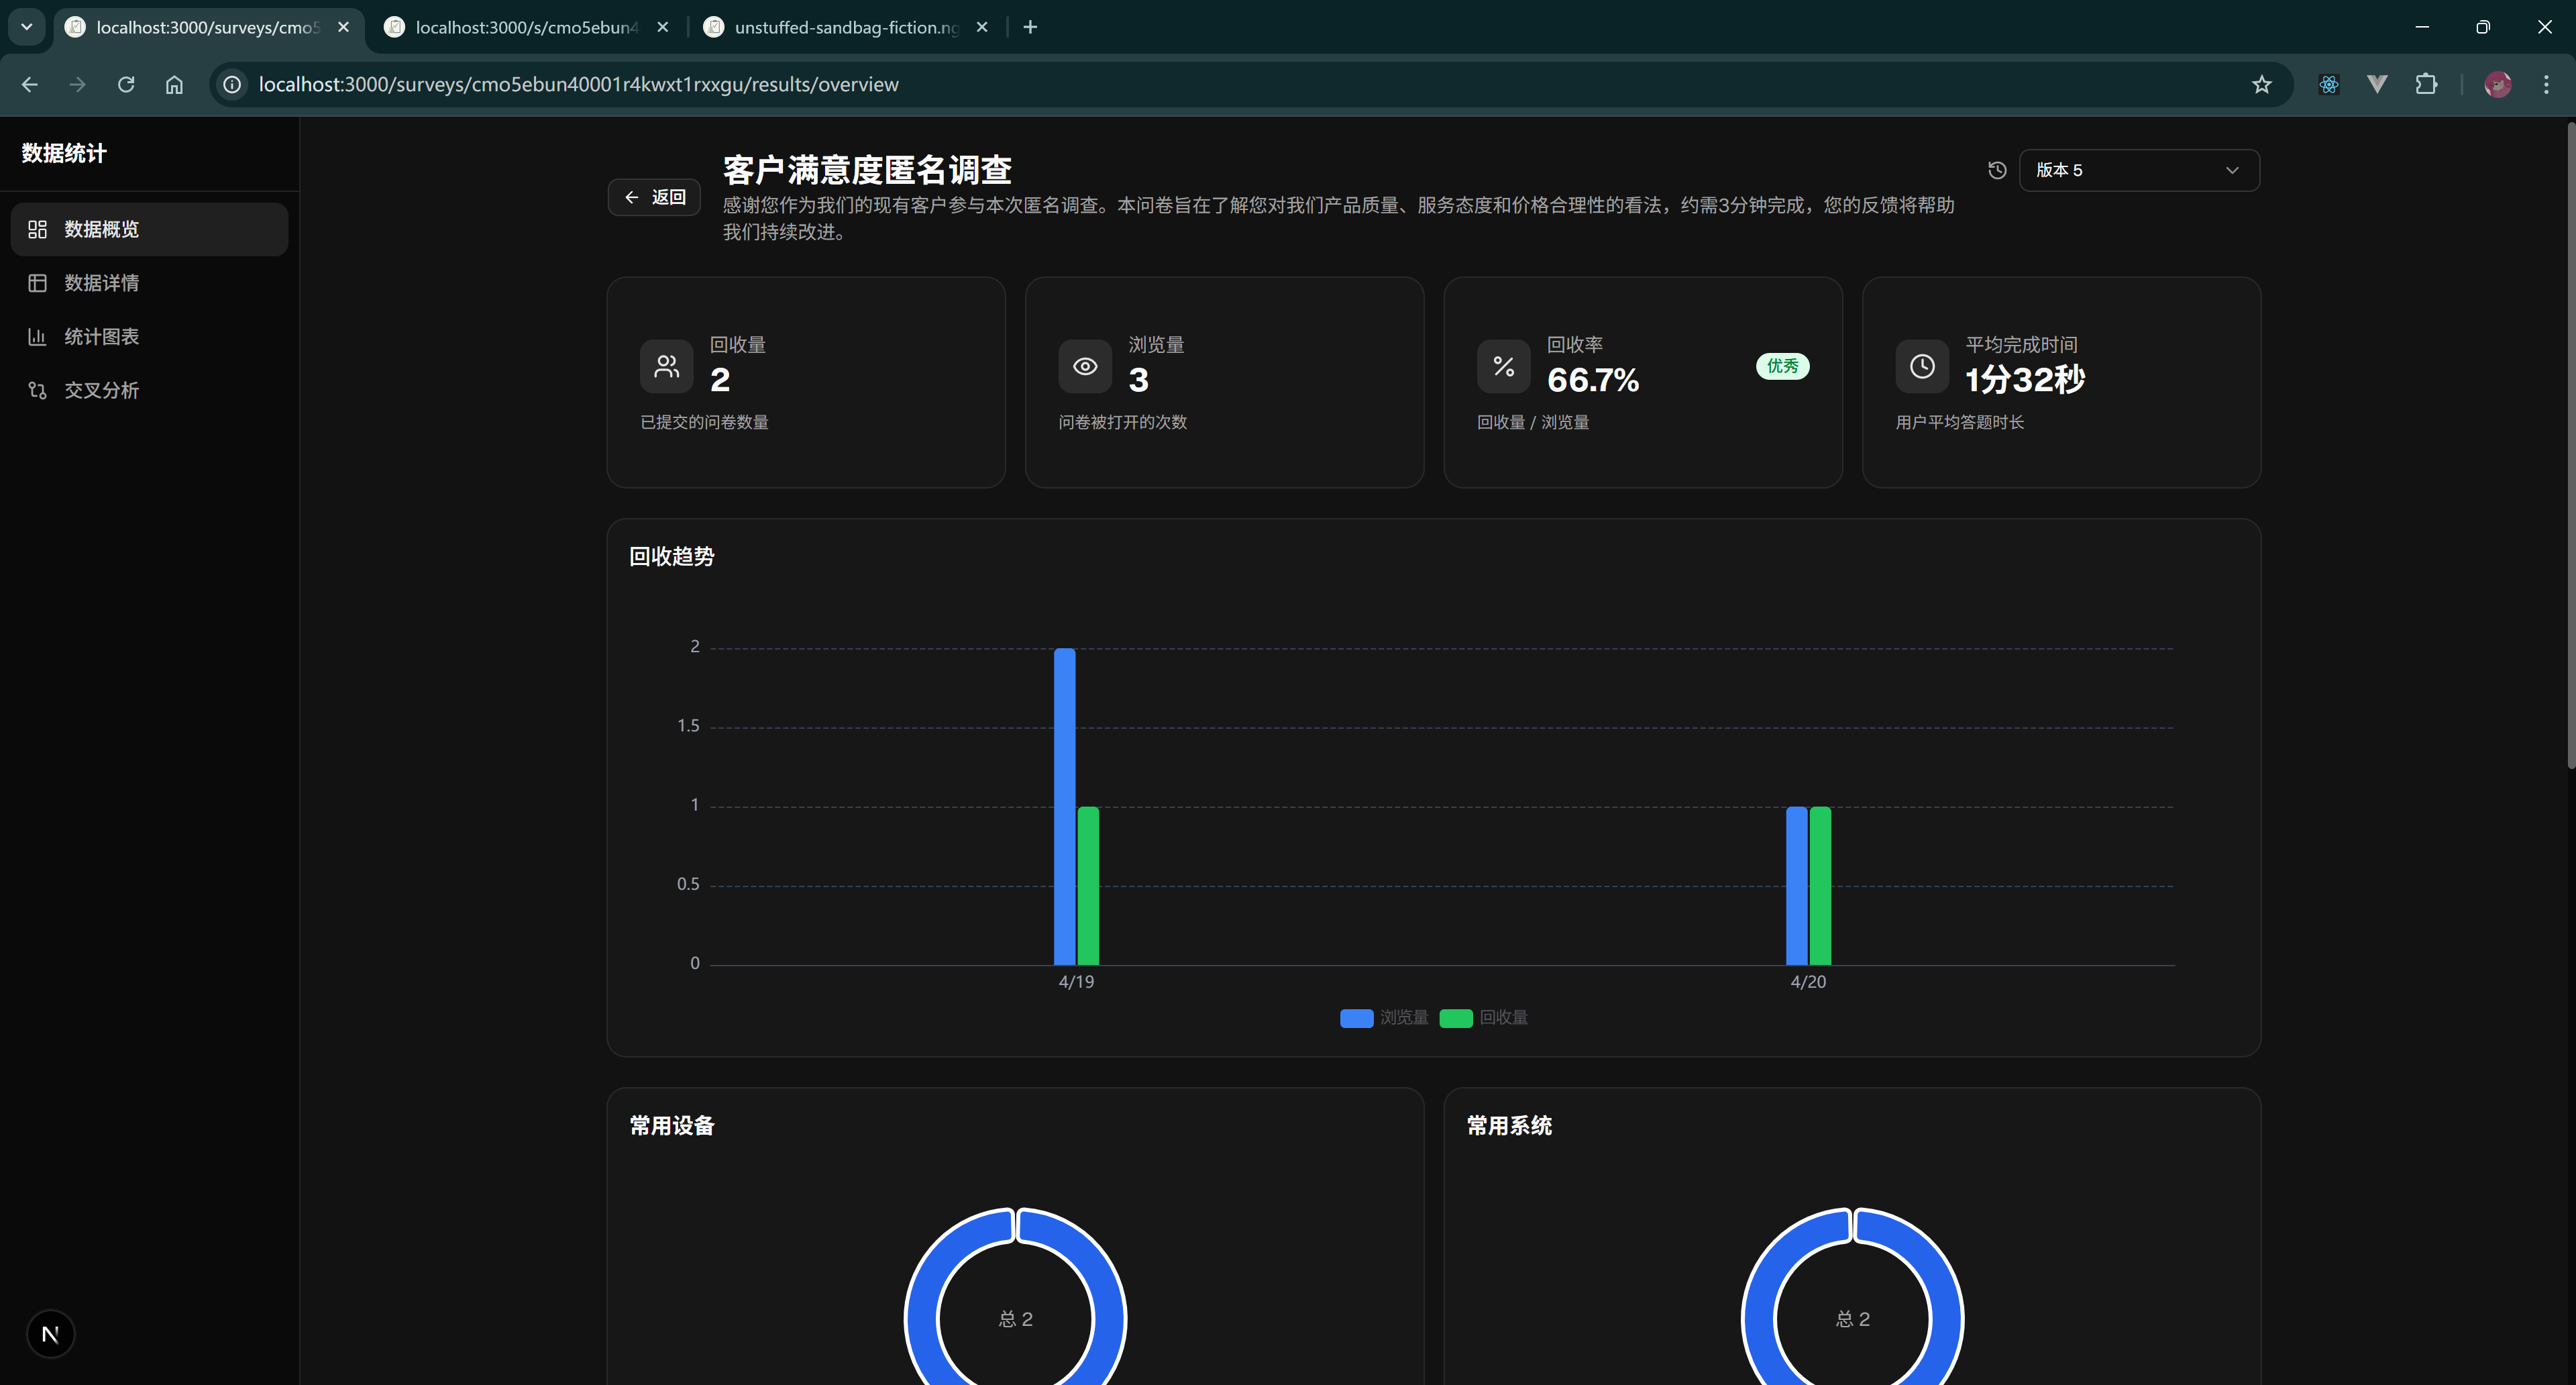
\includegraphics[width=0.95\textwidth]{figures/screenshot-results.png}
\caption{结果统计页面}
\end{figure}

\section{附录 C：项目结构}

\begin{minted}[linenos]{bash}
survey-test/
├── app/                    # Next.js App Router
│   ├── (auth)/            # 认证路由组
│   ├── (dashboard)/       # 仪表盘路由组
│   ├── (editor)/          # 编辑器路由组
│   ├── api/               # API 路由
│   ├── s/[token]/         # 公开问卷页面
│   └── invite/            # 邀请页面
├── components/            # React 组件
│   ├── auth/              # 认证组件
│   ├── editor/            # 编辑器组件
│   ├── questions/         # 题型组件
│   ├── ai/                # AI 组件
│   └── collaboration/     # 协作组件
├── lib/                   # 工具库
│   ├── auth.ts            # 认证配置
│   ├── editor-store.ts    # 编辑器状态
│   ├── questions/         # 题型系统
│   └── ai/                # AI 相关
├── hooks/                 # 自定义 Hooks
├── prisma/                # Prisma 配置
│   └── schema/            # 数据模型
├── docs/                  # 项目文档
├── thesis/                # 毕业论文
└── package.json           # 项目配置
\end{minted}
\captionof{listing}{项目目录结构}
